\documentclass[../main/NEMO_manual]{subfiles}

\begin{document}

\chapter{Time Domain}
\label{chap:TD}

\thispagestyle{plain}

\chaptertoc

\paragraph{Changes record} ~\\

{\footnotesize
  \begin{tabularx}{0.5\textwidth}{l||X|X}
    Release          & Author(s)                                       &
    Modifications                                                      \\
    \hline
    {\em        4.0} & {\em J\'{e}r\^{o}me Chanut \newline Tim Graham} &
    {\em Review \newline Update                                      } \\
    {\em        3.6} & {\em Christian \'{E}th\'{e}                   } &
    {\em Update                                                      } \\
    {\em $\leq$ 3.4} & {\em Gurvan Madec                             } &
    {\em First version                                               } \\
  \end{tabularx}
}

\clearpage

% Missing things:
% - daymod: definition of the time domain (nit000, nitend and the calendar)

\cmtgm{STEVEN :maybe a picture of the directory structure in the introduction which
could be referred to here, would help  ==> to be added}

Having defined the continuous equations in \autoref{chap:MB},
we need now to choose a time discretization,
a key feature of an ocean model as it exerts a strong influence on the structure of the computer code
(\ie\ on its flowchart).
In the present chapter, we provide a general description of the \NEMO\ time stepping strategy and
the consequences for the order in which the equations are solved.

%% =================================================================================================
\section{Time stepping environment}
\label{sec:TD_environment}

The time stepping used in \NEMO\ is a three level scheme that can be represented as follows:
\begin{equation}
  \label{eq:TD}
  x^{t + \rdt} = x^{t - \rdt} + 2 \, \rdt \ \text{RHS}_x^{t - \rdt, \, t, \, t + \rdt}
\end{equation}
where $x$ stands for $u$, $v$, $T$ or $S$;
RHS is the \textbf{R}ight-\textbf{H}and-\textbf{S}ide of the corresponding time evolution equation;
$\rdt$ is the time step;
and the superscripts indicate the time at which a quantity is evaluated.
Each term of the RHS is evaluated at a specific time stepping depending on
the physics with which it is associated.

The choice of the time stepping used for this evaluation is discussed below as well as
the implications for starting or restarting a model simulation.
Note that the time stepping calculation is generally performed in a single operation.
With such a complex and nonlinear system of equations it would be dangerous to
let a prognostic variable evolve in time for each term separately.

The three level scheme requires three arrays for each prognostic variable.
For each variable $x$ there is $x_b$ (before), $x_n$ (now) and $x_a$.
The third array, although referred to as $x_a$ (after) in the code,
is usually not the variable at the after time step;
but rather it is used to store the time derivative (RHS in \autoref{eq:TD})
prior to time-stepping the equation.
The time stepping itself is performed once at each time step where
implicit vertical diffusion is computed,
\ie\ in the \mdl{trazdf} and \mdl{dynzdf} modules.

%% =================================================================================================
\section{Non-diffusive part --- Leapfrog scheme}
\label{sec:TD_leap_frog}

The time stepping used for processes other than diffusion is
the well-known \textbf{L}eap\textbf{F}rog (LF) scheme \citep{mesinger.arakawa_bk76}.
This scheme is widely used for advection processes in low-viscosity fluids.
It is a time centred scheme, \ie\ the RHS in \autoref{eq:TD} is evaluated at
time step $t$, the now time step.
It may be used for momentum and tracer advection, pressure gradient, and Coriolis terms,
but not for diffusion terms.
It is an efficient method that achieves second-order accuracy with
just one right hand side evaluation per time step.
Moreover, it does not artificially damp linear oscillatory motion
nor does it produce instability by amplifying the oscillations.
These advantages are somewhat diminished by the large phase-speed error of the leapfrog scheme,
and the unsuitability of leapfrog differencing for the representation of diffusion and
Rayleigh damping processes.
However, the scheme allows the coexistence of a numerical and a physical mode due to
its leading third order dispersive error.
In other words a divergence of odd and even time steps may occur.
To prevent it, the leapfrog scheme is often used in association with
a \textbf{R}obert-\textbf{A}sselin time filter (hereafter the LF-RA scheme).
This filter,
first designed by \citet{robert_JMSJ66} and more comprehensively studied by \citet{asselin_MWR72},
is a kind of laplacian diffusion in time that mixes odd and even time steps:
\begin{equation}
  \label{eq:TD_asselin}
  x_F^t = x^t + \gamma \, \lt[ x_F^{t - \rdt} - 2 x^t + x^{t + \rdt} \rt]
\end{equation}
where the subscript $F$ denotes filtered values and $\gamma$ is the Asselin coefficient.
$\gamma$ is initialized as \np{rn_atfp}{rn\_atfp} (namelist parameter).
Its default value is \np[=10.e-3]{rn_atfp}{rn\_atfp} (see \autoref{sec:TD_mLF}),
causing only a weak dissipation of high frequency motions (\citep{farge-coulombier_phd87}).
The addition of a time filter degrades the accuracy of the calculation from second to first order.
However, the second order truncation error is proportional to $\gamma$, which is small compared to 1.
Therefore, the LF-RA is a quasi second order accurate scheme.
The LF-RA scheme is preferred to other time differencing schemes such as
predictor corrector or trapezoidal schemes, because the user has an explicit and simple control of
the magnitude of the time diffusion of the scheme.
When used with the 2$^nd$ order space centred discretisation of the advection terms in
the momentum and tracer equations, LF-RA avoids implicit numerical diffusion:
diffusion is set explicitly by the user through the Robert-Asselin filter parameter and
the viscosity and diffusion coefficients.

%% =================================================================================================
\section{Diffusive part --- Forward or backward scheme}
\label{sec:TD_forward_imp}

The leapfrog differencing scheme is unsuitable for
the representation of diffusion and damping processes.
For a tendency $D_x$, representing a diffusion term or a restoring term to a tracer climatology
(when present, see \autoref{sec:TRA_dmp}), a forward time differencing scheme is used :
\[
  %\label{eq:TD_euler}
  x^{t + \rdt} = x^{t - \rdt} + 2 \, \rdt \ D_x^{t - \rdt}
\]

This is diffusive in time and conditionally stable.
The conditions for stability of second and fourth order horizontal diffusion schemes are
\citep{griffies_bk04}:
\begin{equation}
  \label{eq:TD_euler_stability}
  A^h <
  \begin{cases}
    \frac{e^2}{ 8 \, \rdt} & \text{laplacian diffusion} \\
    \frac{e^4}{64 \, \rdt} & \text{bilaplacian diffusion}
  \end{cases}
\end{equation}
where $e$ is the smallest grid size in the two horizontal directions and
$A^h$ is the mixing coefficient.
The linear constraint \autoref{eq:TD_euler_stability} is a necessary condition, but not sufficient.
If it is not satisfied, even mildly, then the model soon becomes wildly unstable.
The instability can be removed by either reducing the length of the time steps or
reducing the mixing coefficient.

For the vertical diffusion terms, a forward time differencing scheme can be used,
but usually the numerical stability condition imposes a strong constraint on the time step.
To overcome the stability constraint, a backward (or implicit) time differencing scheme is used.
This scheme is unconditionally stable but diffusive and can be written as follows:
\begin{equation}
  \label{eq:TD_imp}
  x^{t + \rdt} = x^{t - \rdt} + 2 \, \rdt \ \text{RHS}_x^{t + \rdt}
\end{equation}

\cmtgm{UPDATE the next paragraphs with time varying thickness ...}

This scheme is rather time consuming since it requires a matrix inversion.
For example, the finite difference approximation of the temperature equation is:
\[
  % \label{eq:TD_imp_zdf}
  \frac{T(k)^{t + 1} - T(k)^{t - 1}}{2 \; \rdt}
  \equiv
  \text{RHS} + \frac{1}{e_{3t}} \delta_k \lt[ \frac{A_w^{vT}}{e_{3w} } \delta_{k + 1/2} \lt[ T^{t + 1} \rt] \rt]
\]
where RHS is the right hand side of the equation except for the vertical diffusion term.
We rewrite \autoref{eq:TD_imp} as:
\begin{equation}
  \label{eq:TD_imp_mat}
  -c(k + 1) \; T^{t + 1}(k + 1) + d(k) \; T^{t + 1}(k) - \; c(k) \; T^{t + 1}(k - 1) \equiv b(k)
\end{equation}
where
\[
  c(k) = A_w^{vT} (k) \, / \, e_{3w} (k) \text{,} \quad
  d(k) = e_{3t}   (k)       \, / \, (2 \rdt) + c_k + c_{k + 1} \quad \text{and} \quad
  b(k) = e_{3t}   (k) \; \lt( T^{t - 1}(k) \, / \, (2 \rdt) + \text{RHS} \rt)
\]

\autoref{eq:TD_imp_mat} is a linear system of equations with
an associated matrix which is tridiagonal.
Moreover, $c(k)$ and $d(k)$ are positive and
the diagonal term is greater than the sum of the two extra-diagonal terms,
therefore a special adaptation of the Gauss elimination procedure is used to find the solution
(see for example \citet{richtmyer.morton_bk67}).

%% =================================================================================================
\section{Surface pressure gradient}
\label{sec:TD_spg_ts}

The leapfrog environment supports a centred in time computation of the surface pressure,
\ie\ evaluated at \textit{now} time step.
This refers to as the explicit free surface case in the code
(\np[=.true.]{ln_dynspg_exp}{ln\_dynspg\_exp}).
This choice however imposes a strong constraint on the time step which
should be small enough to resolve the propagation of external gravity waves.
As a matter of fact, one rather use in a realistic setup,
a split-explicit free surface (\np[=.true.]{ln_dynspg_ts}{ln\_dynspg\_ts}) in which
barotropic and baroclinic dynamical equations are solved separately with ad-hoc time steps.
The use of the time-splitting (in combination with non-linear free surface) imposes
some constraints on the design of the overall flowchart,
in particular to ensure exact tracer conservation (see \autoref{fig:TD_TimeStep_flowchart}).

Compared to the former use of the filtered free surface in \NEMO\ v3.6 (\citet{roullet.madec_JGR00}),
the use of a split-explicit free surface is advantageous on massively parallel computers.
Indeed, no global computations are anymore required by the elliptic solver which
saves a substantial amount of communication time.
Fast barotropic motions (such as tides) are also simulated with a better accuracy.

%\cmtgm{
\begin{figure}
  \centering
  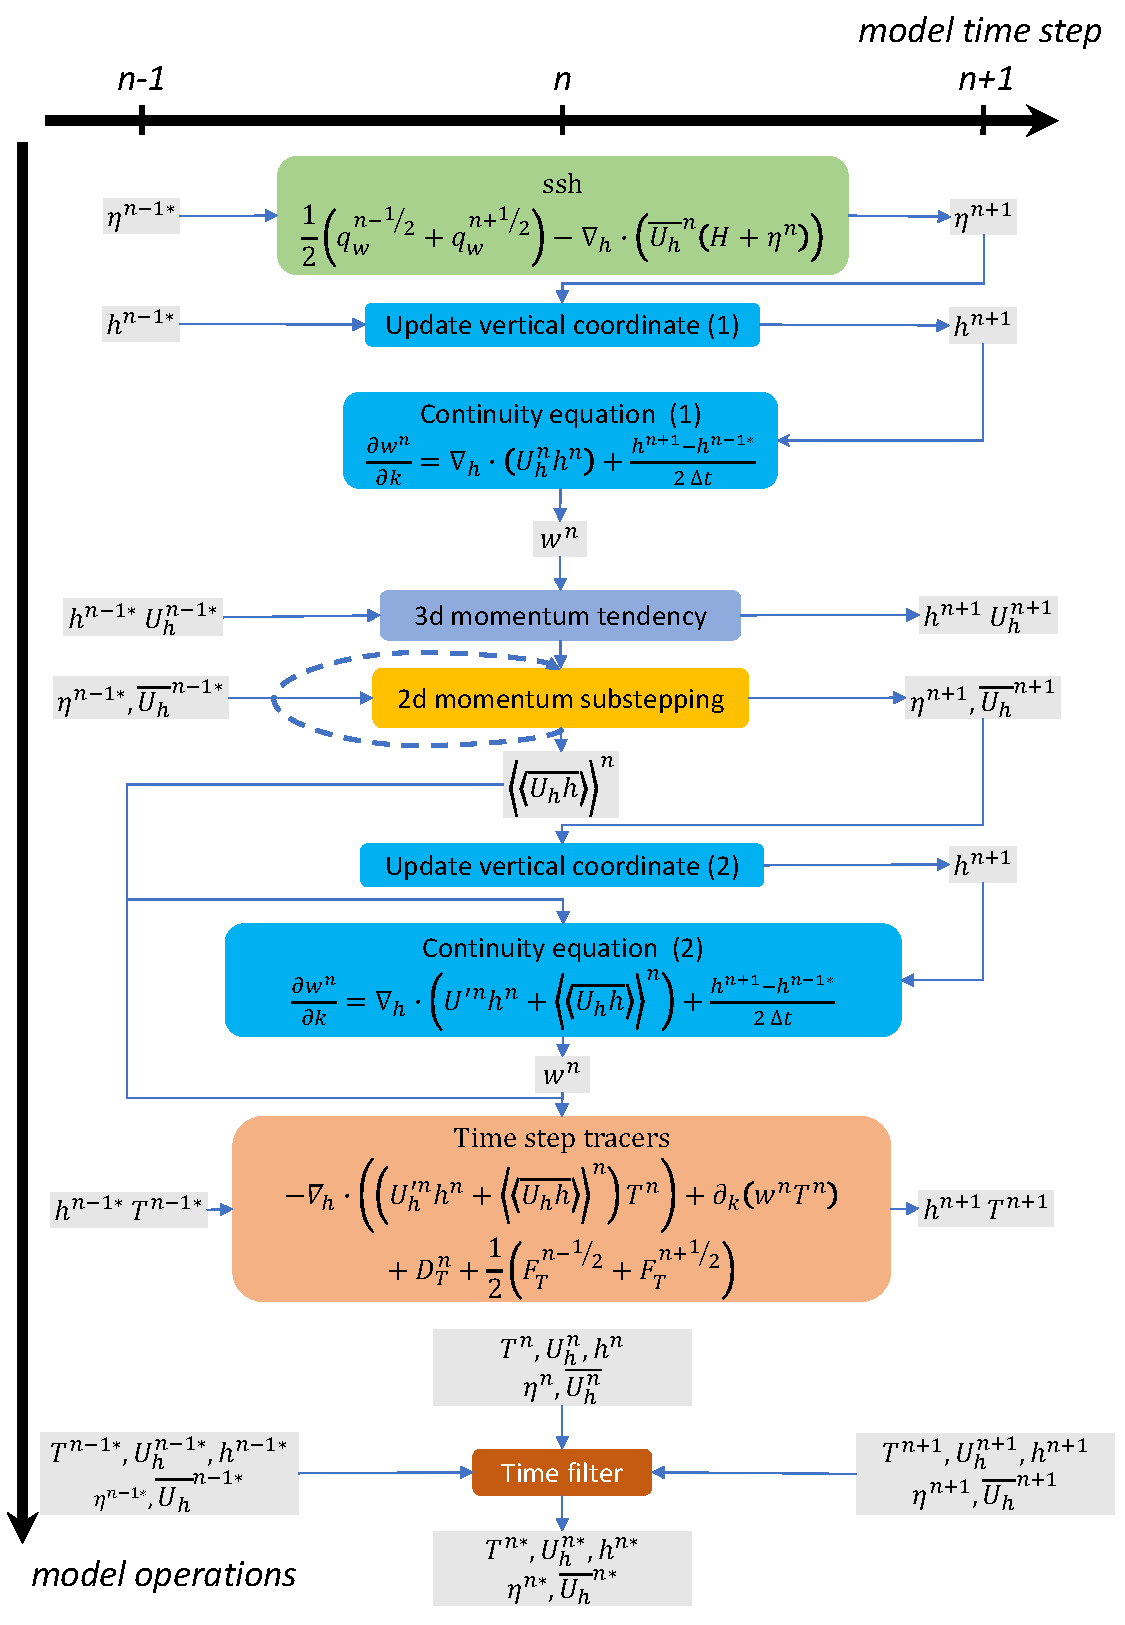
\includegraphics[width=0.66\textwidth]{TD_TimeStepping_flowchart_v4}
  \caption[Leapfrog time stepping sequence with split-explicit free surface]{
    Sketch of the leapfrog time stepping sequence in \NEMO\ with split-explicit free surface.
    The latter combined with non-linear free surface requires
    the dynamical tendency being updated prior tracers tendency to ensure conservation.
    Note the use of time integrated fluxes issued from the barotropic loop in
    subsequent calculations of tracer advection and in the continuity equation.
    Details about the time-splitting scheme can be found in \autoref{subsec:DYN_spg_ts}.}
  \label{fig:TD_TimeStep_flowchart}
\end{figure}
%}

%% =================================================================================================
\section{Modified LeapFrog -- Robert Asselin filter scheme (LF-RA)}
\label{sec:TD_mLF}

Significant changes have been introduced by \cite{leclair.madec_OM09} in
the LF-RA scheme in order to ensure tracer conservation and to
allow the use of a much smaller value of the Asselin filter parameter.
The modifications affect both the forcing and filtering treatments in the LF-RA scheme.

In a classical LF-RA environment,
the forcing term is centred in time, \ie\ it is time-stepped over a $2 \rdt$ period:
$x^t = x^t + 2 \rdt Q^t$ where $Q$ is the forcing applied to $x$,
and the time filter is given by \autoref{eq:TD_asselin} so that
$Q$ is redistributed over several time step.
In the modified LF-RA environment, these two formulations have been replaced by:
\begin{gather}
  \label{eq:TD_forcing}
  x^{t + \rdt} = x^{t - \rdt} + \rdt \lt( Q^{t - \rdt / 2} + Q^{t + \rdt / 2} \rt)  \\
  \label{eq:TD_RA}
  x_F^t       = x^t + \gamma \, \lt( x_F^{t - \rdt} - 2 x^t + x^{t + \rdt} \rt)
                    - \gamma \, \rdt \, \lt( Q^{t + \rdt / 2} - Q^{t - \rdt / 2} \rt)
\end{gather}
The change in the forcing formulation given by \autoref{eq:TD_forcing}
(see \autoref{fig:TD_MLF_forcing}) has a significant effect:
the forcing term no longer excites the divergence of odd and even time steps
\citep{leclair.madec_OM09}.
% forcing seen by the model....
This property improves the LF-RA scheme in two aspects.
First, the LF-RA can now ensure the local and global conservation of tracers.
Indeed, time filtering is no longer required on the forcing part.
The influence of the Asselin filter on the forcing is explicitly removed by
adding a new term in the filter (last term in \autoref{eq:TD_RA} compared to \autoref{eq:TD_asselin}).
Since the filtering of the forcing was the source of non-conservation in the classical LF-RA scheme,
the modified formulation becomes conservative \citep{leclair.madec_OM09}.
Second, the LF-RA becomes a truly quasi-second order scheme.
Indeed, \autoref{eq:TD_forcing} used in combination with a careful treatment of static instability
(\autoref{subsec:ZDF_evd}) and of the TKE physics (\autoref{subsec:ZDF_tke_ene})
(the two other main sources of time step divergence),
allows a reduction by two orders of magnitude of the Asselin filter parameter.

Note that the forcing is now provided at the middle of a time step:
$Q^{t + \rdt / 2}$ is the forcing applied over the $[t,t + \rdt]$ time interval.
This and the change in the time filter, \autoref{eq:TD_RA},
allows for an exact evaluation of the contribution due to the forcing term between any two time steps,
even if separated by only $\rdt$ since the time filter is no longer applied to the forcing term.

\begin{figure}
  \centering
  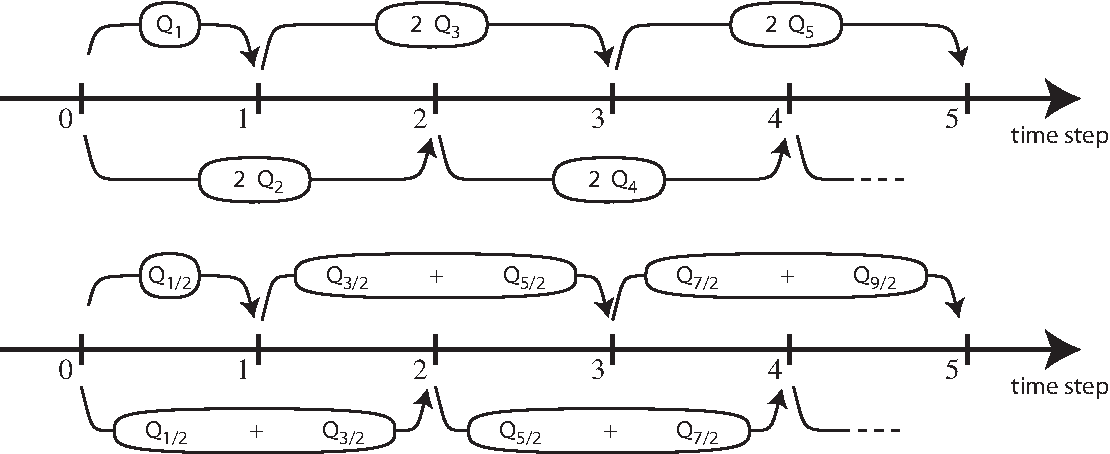
\includegraphics[width=0.66\textwidth]{TD_MLF_forcing}
  \caption[Forcing integration methods for modified leapfrog (top and bottom)]{
    Illustration of forcing integration methods.
    (top) ''Traditional'' formulation:
    the forcing is defined at the same time as the variable to which it is applied
    (integer value of the time step index) and it is applied over a $2 \rdt$ period.
    (bottom)  modified formulation:
    the forcing is defined in the middle of the time
    (integer and a half value of the time step index) and
    the mean of two successive forcing values ($n - 1 / 2$, $n + 1 / 2$) is applied over
    a $2 \rdt$ period.}
  \label{fig:TD_MLF_forcing}
\end{figure}

%% =================================================================================================
\section{Start/Restart strategy}
\label{sec:TD_rst}

\begin{listing}
  \nlst{namrun}
  \caption{\forcode{&namrun}}
  \label{lst:namrun}
\end{listing}

The first time step of this three level scheme when starting from initial conditions is
a forward step (Euler time integration):
\[
  % \label{eq:TD_DOM_euler}
  x^1 = x^0 + \rdt \ \text{RHS}^0
\]
This is done simply by keeping the leapfrog environment
(\ie\ the \autoref{eq:TD} three level time stepping) but
setting all $x^0$ (\textit{before}) and $x^1$ (\textit{now}) fields equal at the first time step and
using half the value of a leapfrog time step ($2 \rdt$).

It is also possible to restart from a previous computation, by using a restart file.
The restart strategy is designed to ensure perfect restartability of the code:
the user should obtain the same results to machine precision either by
running the model for $2N$ time steps in one go,
or by performing two consecutive experiments of $N$ steps with a restart.
This requires saving two time levels and many auxiliary data in
the restart files in machine precision.

Note that the time step $\rdt$, is also saved in the restart file.
When restarting, if the time step has been changed, or
one of the prognostic variables at \textit{before} time step is missing,
an Euler time stepping scheme is imposed.
A forward initial step can still be enforced by the user by
setting the namelist variable \np[=0]{nn_euler}{nn\_euler}.
Other options to control the time integration of the model are defined through
the \nam{run}{run} namelist variables.

\cmtgm{
add here how to force the restart to contain only one time step for operational purposes

add also the idea of writing several restart for seasonal forecast : how is it done ?

verify that all namelist parameters are truly described

a word on the check of restart  .....
}

\cmtgm{       % add a subsection here

%% =================================================================================================
\subsection{Time domain}
\label{subsec:TD_time}

Options are defined through the\nam{dom}{dom} namelist variables.
 \colorbox{yellow}{add here a few word on nit000 and nitend}

 \colorbox{yellow}{Write documentation on the calendar and the key variable adatrj}

add a description of daymod, and the model calendar (leap-year and co)

}     %% end add

\cmtgm{       % add implicit in vvl case  and Crant-Nicholson scheme

Implicit time stepping in case of variable volume thickness.

Tracer case (NB for momentum in vector invariant form take care!)

\begin{flalign*}
  &\frac{\lt( e_{3t}\,T \rt)_k^{t+1}-\lt( e_{3t}\,T \rt)_k^{t-1}}{2\rdt}
  \equiv \text{RHS}+ \delta_k \lt[ {\frac{A_w^{vt} }{e_{3w}^{t+1} }\delta_{k + 1/2} \lt[ {T^{t+1}} \rt]}
  \rt]      \\
  &\lt( e_{3t}\,T \rt)_k^{t+1}-\lt( e_{3t}\,T \rt)_k^{t-1}
  \equiv {2\rdt} \ \text{RHS}+ {2\rdt} \ \delta_k \lt[ {\frac{A_w^{vt} }{e_{3w}^{t+1} }\delta_{k + 1/2} \lt[ {T^{t+1}} \rt]}
  \rt]      \\
  &\lt( e_{3t}\,T \rt)_k^{t+1}-\lt( e_{3t}\,T \rt)_k^{t-1}
  \equiv 2\rdt \ \text{RHS}
  + 2\rdt \ \lt\{ \lt[ \frac{A_w^{vt}}{e_{3w}^{t+1}} \rt]_{k + 1/2} [ T_{k +1}^{t+1} - T_k      ^{t+1} ]
    - \lt[ \frac{A_w^{vt}}{e_{3w}^{t+1}} \rt]_{k - 1/2} [ T_k       ^{t+1} - T_{k -1}^{t+1} ]  \rt\}     \\
  &\\
  &\lt( e_{3t}\,T \rt)_k^{t+1}
  -  {2\rdt} \           \lt[ \frac{A_w^{vt}}{e_{3w}^{t+1}} \rt]_{k + 1/2}                  T_{k +1}^{t+1}
  + {2\rdt} \ \lt\{  \lt[ \frac{A_w^{vt}}{e_{3w}^{t+1}} \rt]_{k + 1/2}
    +  \lt[ \frac{A_w^{vt}}{e_{3w}^{t+1}} \rt]_{k - 1/2}     \rt\}   T_{k    }^{t+1}
  -  {2\rdt} \           \lt[ \frac{A_w^{vt}}{e_{3w}^{t+1}} \rt]_{k - 1/2}                  T_{k -1}^{t+1}      \\
  &\equiv \lt( e_{3t}\,T \rt)_k^{t-1} + {2\rdt} \ \text{RHS}    \\
  %
\end{flalign*}
\begin{flalign*}
  \allowdisplaybreaks
  \intertext{ Tracer case }
  %
  &  \qquad \qquad  \quad   -  {2\rdt}                  \ \lt[ \frac{A_w^{vt}}{e_{3w}^{t+1}} \rt]_{k + 1/2}
  \qquad \qquad \qquad  \qquad  T_{k +1}^{t+1}   \\
  &+ {2\rdt} \ \biggl\{  (e_{3t})_{k   }^{t+1}  \bigg. +    \lt[ \frac{A_w^{vt}}{e_{3w}^{t+1}} \rt]_{k + 1/2}
  +   \lt[ \frac{A_w^{vt}}{e_{3w}^{t+1}} \rt]_{k - 1/2} \bigg. \biggr\}  \ \ \ T_{k   }^{t+1}  &&\\
  & \qquad \qquad  \qquad \qquad \qquad \quad \ \ -  {2\rdt} \                          \lt[ \frac{A_w^{vt}}{e_{3w}^{t+1}} \rt]_{k - 1/2}                          \quad \ \ T_{k -1}^{t+1}
  \ \equiv \ \lt( e_{3t}\,T \rt)_k^{t-1} + {2\rdt} \ \text{RHS}  \\
  %
\end{flalign*}
\begin{flalign*}
  \allowdisplaybreaks
  \intertext{ Tracer content case }
  %
  & -  {2\rdt} \              & \frac{(A_w^{vt})_{k + 1/2}} {(e_{3w})_{k + 1/2}^{t+1}\;(e_{3t})_{k +1}^{t+1}}  && \  \lt( e_{3t}\,T \rt)_{k +1}^{t+1}   &\\
  & + {2\rdt} \ \lt[ 1  \rt.+ & \frac{(A_w^{vt})_{k + 1/2}} {(e_{3w})_{k + 1/2}^{t+1}\;(e_{3t})_k^{t+1}}
  + & \frac{(A_w^{vt})_{k - 1/2}} {(e_{3w})_{k - 1/2}^{t+1}\;(e_{3t})_k^{t+1}}  \lt.  \rt]  & \lt( e_{3t}\,T \rt)_{k   }^{t+1}  &\\
  & -  {2\rdt} \               & \frac{(A_w^{vt})_{k - 1/2}} {(e_{3w})_{k - 1/2}^{t+1}\;(e_{3t})_{k -1}^{t+1}}     &\  \lt( e_{3t}\,T \rt)_{k -1}^{t+1}
  \equiv \lt( e_{3t}\,T \rt)_k^{t-1} + {2\rdt} \ \text{RHS}  &
\end{flalign*}

}

\subinc{\input{../../global/epilogue}}

\end{document}
